\documentclass{article}
\usepackage{amsmath}
\usepackage{amsfonts}
\usepackage{amssymb}
\usepackage{mathrsfs}
\usepackage{cancel}

\usepackage{graphicx}


\setlength\parindent{0pt}

\author{Pranav Tikkawar}
\title{TODO}

\begin{document}
\maketitle

\section{Section 1}
\begin{figure}[ht]
    \centering
    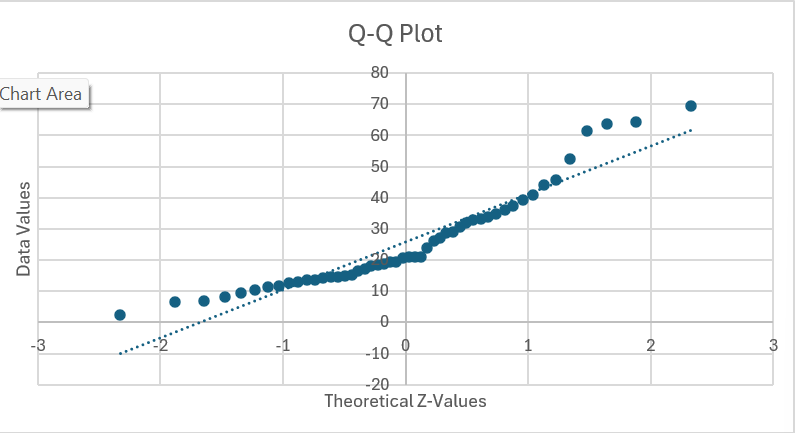
\includegraphics[width=0.8\textwidth]{A3img/Q-QPlot.png}
    \caption{Q-Q Plot}
    \label{fig:qq_plot}
\end{figure}

\section{Section 2}
I believe that the Q-Q plot is relatively linear and thus approximately normal. Despite that, I can also see it being somewhat right skewed as it matches the profile given in the slide/lectures. Nonetheless, it seems normal. 

\section{Section 3}
To determine how likely they are to come to the correct conclusion to reject the null hypothesis, we need to calculate the power of the test. The power of the test is the probability of correctly rejecting the null hypothesis when the alternative hypothesis is true. In this case, the alternative hypothesis is that the mean amount spent per shopping trip at the Quartz Emporium is not equal to \$23.00.\\
Thus the formula for the power of the test is given by:
\begin{equation}
    \text{Power} = 1 - \Phi\left( \text(z_{val}) - \text(z_{score}) \right) 
\end{equation}
Where Zval is the z-score for the level of significance, and Zscore is the z-score for the alternative hypothesis. $\Phi$ is the normal distribution function.\\
The z-score for the level of significance is given by:
\begin{equation}
    z_{val} = \Phi^{-1}\left(1 - \alpha\right)
\end{equation}
Where $\alpha$ is the level of significance.\\
The z-score for the alternative hypothesis is given by:
\begin{equation}
    z_{score} = \frac{\bar{x} - \mu}{\frac{\sigma}{\sqrt{n}}}
\end{equation}
Where $\bar{x}$ is the sample mean, $\mu$ is the population mean, $\sigma$ is the population standard deviation, and n is the sample size.\\
Given that the population mean is \$23.00, the population standard deviation is \$16.00, the sample mean is \$22.50, the sample size is 50, and the level of significance is 0.05, we can calculate the power of the test as follows:
\begin{equation}
    z_{val} = \Phi^{-1}\left(1 - 0.05\right) = \Phi^{-1}\left(0.95\right) \approx 1.645
\end{equation}
\begin{equation}
    z_{score} = \frac{22.50 - 23.00}{\frac{16.00}{\sqrt{50}}} = \frac{-0.50}{2.2627} \approx -0.221
\end{equation}
\begin{equation}
    \text{Power} = 1 - \Phi\left(1.645 - 0.221\right) = 1 - \Phi\left(1.424\right) \approx 0.077
\end{equation}
Therefore, the WatchDogs are .07724 likely to come to the correct conclusion to reject the null hypothesis if in fact the mean amount spent per shopping trip at the Quartz Emporium is \$23.00.

\section{Section 4}
To determine the probability that WatchDogs could come to the erroneous conclusion to accept the null hypothesis, we need to calculate the probability of Type II error. The probability of Type II error is the probability of failing to reject the null hypothesis when the alternative hypothesis is true. In this case, the alternative hypothesis is that the mean amount spent per shopping trip at the Quartz Emporium is not equal to \$23.00.\\
We can quickly calculate the probability of Type II error by subtracting the power of the test from 1.\\
Given that the power of the test is 0.077, we can calculate the probability of Type II error as follows:
\begin{equation}
    \text{Probability of Type II Error} = 1 - \text{Power} = 1 - 0.07724 = 0.92276
\end{equation}
Therefore, the WatchDogs are 0.92276 likely to come to the erroneous conclusion to accept the null hypothesis if in fact the mean amount spent per shopping trip at the Quartz Emporium is \$23.00.

\section{Section 5}
To determine how many shoppers from the Quartz Emporium the WatchDogs should survey to be 80\% certain they will come to the correct conclusion to reject the null hypothesis, we need to calculate the sample size. The sample size is given by:
\begin{equation}
    n = \left( \frac{z_{\alpha} + z_{\beta}}{\text{effect size}} \right)^2
\end{equation}
Where $z_{\alpha}$ is the z-score for the level of significance, $z_{\beta}$ is the z-score for the power of the test, and the effect size is given by:
\begin{equation}
    \text{effect size} = \frac{\mu - \bar{x}}{\sigma}
\end{equation}
Given that the population mean is \$23.00, the population standard deviation is \$16.00, the sample mean is \$22.50, the level of significance is 0.05, and the power of the test is 0.80, we can calculate the sample size.\\
We would need a sample size of 6331 shoppers from the Quartz Emporium to be 80\% certain that the WatchDogs will come to the correct conclusion to reject the null hypothesis.



\end{document}